% =====================================================================
% AI251P Applied Computer Vision -- Smart Pet Vision, Phase 2 (M4/M5/M8)
% Styled directly from the team's submitted Phase 1 Overleaf source.
% Rebuild: latexmk -pdf -interaction=nonstopmode main.tex
% All quantitative results are attributed to saved evidence; no new training.
% =====================================================================
\documentclass[11pt,a4paper]{article}
\usepackage[T1]{fontenc}
\usepackage[utf8]{inputenc}
\usepackage{mathpazo}
\usepackage[margin=2.2cm]{geometry}
\usepackage{booktabs,tabularx,array,multirow,longtable}
\usepackage{graphicx}
\usepackage{caption}
\usepackage{enumitem}
\usepackage{amssymb}
\usepackage{xcolor}
\usepackage{fancyhdr}
\usepackage{float,placeins,microtype,xurl}
\usepackage[colorlinks=true,linkcolor=blue!50!black,urlcolor=blue!50!black]{hyperref}
\hypersetup{pdftitle={Smart Pet Vision - Phase 2 Report},pdfauthor={Smart Pet Vision Team},pdfsubject={AI251P Applied Computer Vision - Capstone Phase 2},pdflang={en-US}}
\newcommand{\teamname}{Smart Pet Vision}
\newcommand{\projecttitle}{Smart Pet Vision: Detection, Segmentation and Staff-Review Integration}
\newcommand{\pts}[1]{\texorpdfstring{\hfill{\normalsize\mdseries(#1 points)}}{}}
\newlist{checklist}{itemize}{1}
\setlist[checklist]{label=$\square$,leftmargin=1.6em,itemsep=2pt}
\newcolumntype{Y}{>{\raggedright\arraybackslash}X}
\newcolumntype{P}[1]{>{\raggedright\arraybackslash}p{#1}}
\renewcommand{\arraystretch}{1.21}
\setlength{\parindent}{0pt}
\setlength{\parskip}{4pt}
\renewcommand{\ttdefault}{lmtt}
\emergencystretch=2em
\captionsetup{font=small,labelfont=bf}
\newcommand{\code}[1]{\path{#1}}
\pagestyle{fancy}\fancyhf{}
\lhead{\small\itshape AI251P Applied Computer Vision}
\rhead{\small\itshape Phase 2 -- \teamname}
\cfoot{\thepage}
\setlength{\headheight}{14pt}
\begin{document}
\begin{center}
{\large AI251P Applied Computer Vision}\\[4pt]
{\LARGE\bfseries Capstone Project -- Phase 2 Report}\\[6pt]
{\Large \projecttitle}\\[4pt]
\teamname\ \textperiodcentered\ Phase 2 (M4, M5, M8; 45 points)\\[2pt]
Due 15 November 2026
\end{center}

\section{Team and project}

{\small\begin{tabularx}{\linewidth}{@{}P{3cm} Y@{}}\toprule
Field & Details\\\midrule
Team name & Smart Pet Vision\\
Application area & Animal welfare; preparing cat/dog adoption photographs for staff review\\
Primary task & Full-body detection, animal segmentation, species verification and review referral\\
Repository & \url{https://github.com/Yasser-20-alhajlah/smart-pet-vision} Phase 1 code in \code{smart-pet-vision/}; Phase 2 code in \code{smart-pet-vision/phase2/} (see Section~\ref{sec:repro})\\
Experiment tracking & \url{https://wandb.ai/yasser-alhajlah-kaust/smart-pet-vision}\\
Report basis & Frozen Phase 1 report, archived Phase 2 evaluation and verified 30 October source snapshot\\
\bottomrule\end{tabularx}}
\subsection*{Team members}

{\small\begin{tabularx}{\linewidth}{@{}P{3.3cm} P{1.5cm} P{2.6cm} Y@{}}\toprule
Name & Student ID & Workstream & Phase 2 responsibility\\\midrule
Abdulrahman Mastour Alharthi & 225478 & Data/class. & Label integrity, dataset provenance, species verification and evaluation\\
Yasser Mansour Alhajlah & 225481 & Detection & Body annotations, YOLO detector, thresholds, galleries and video\\
Mohammed Adeeb Alrashdi & 225488 & Segmentation & Trimap masks, SAM reference, YOLO segmentation and mask analysis\\
Musaad Obaied Saad Alqahtani & 225471 & Integration & Manifest, end-to-end pipeline, HTTP service, export and benchmarking\\
\bottomrule\end{tabularx}}
\subsection*{Problem and acceptance criteria}
\begin{itemize}[leftmargin=1.2em,itemsep=1pt]
\item \textbf{Input $\rightarrow$ output:} A photograph $\rightarrow$ animal boxes, selected cat/dog verification, a matched body mask and a technical \emph{ready / refer-to-staff} verdict.
\item \textbf{Intended decision:} Help shelter staff assess listing photos; \textbf{every image requires staff approval}. A technical \emph{ready} verdict never authorises automatic publication.
\item \textbf{Module goals:} M4 reports detection accuracy and failure modes; M5 measures masks against ground truth; M8 integrates models and evaluates deployment behaviour.
\item \textbf{Evidence policy:} Held-out Oxford evaluations, supplementary team-photo results, recorded T4/CPU benchmarks and saved verification checks are labelled by source and evaluation setting. This report preserves the established measurements without retraining.
\end{itemize}
\clearpage

\section{Object detection (M4)\pts{15}}
\subsection{Dataset and body-box annotations}
Oxford-IIIT Pet provides image classes and trimaps. Full-body boxes were derived by enclosing the foreground plus border, rather than using the source head boxes. The cleaned set contains \textbf{7,335 images} (2,366 cats and 4,969 dogs), grouped to avoid documented exact/near-duplicate split crossing; training/validation/test sizes are \textbf{5,123 / 1,106 / 1,106} (seed 42). Four loose body boxes were found among 300 reviewed, with no missing animal in that review. The separate, private team set has 401 photos and 503 annotated animal boxes.

YOLO-format labels were verified by pixel-coordinate round-trip on 7,335 labels: zero missing labels, zero class mismatches and a maximum reported rounding difference of 0.0009 pixels. This is an annotation-integrity check, not a measure of detector quality.
\begin{figure}[H]\centering
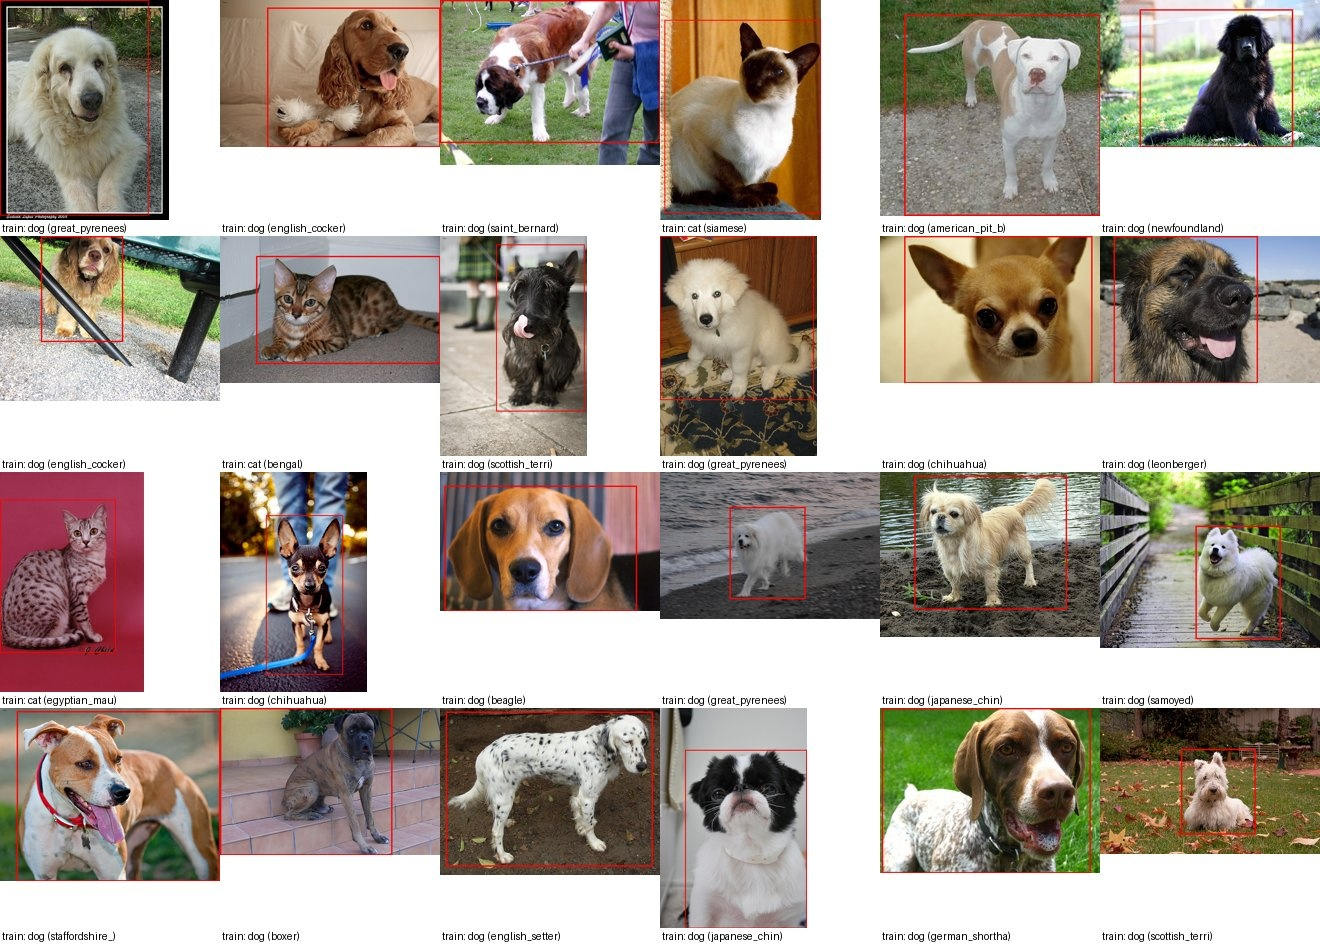
\includegraphics[width=.88\linewidth,height=7.5cm,keepaspectratio]{figures/M4_yolo_label_check.jpg}
\caption{Body-box annotation review examples. Data split: Oxford train; image resolution: native; box overlay from verified YOLO labels; confidence threshold: not applicable.}
\end{figure}
\subsection{Training protocol}
A \textbf{YOLO11s} detector was fine-tuned for 40 epochs at 640-pixel input on the training split. The recorded training run is \href{https://wandb.ai/yasser-alhajlah-kaust/smart-pet-vision/runs/2seovilv}{W\&B 2seovilv}. Checkpoint and threshold selection are tied to validation rather than the test split. Training was carried out historically; this document reuses recorded artifacts without retraining.
\clearpage

\subsection{Operating-point selection}
Validation swept confidence thresholds 0.05--0.70 and NMS IoU values 0.50--0.70. The recorded rule maximised F1 subject to recall $\geq0.80$. It selected \textbf{confidence 0.40, NMS IoU 0.50}: validation precision 0.9592, recall 0.9566 and F1 0.9579.
\begin{figure}[H]\centering
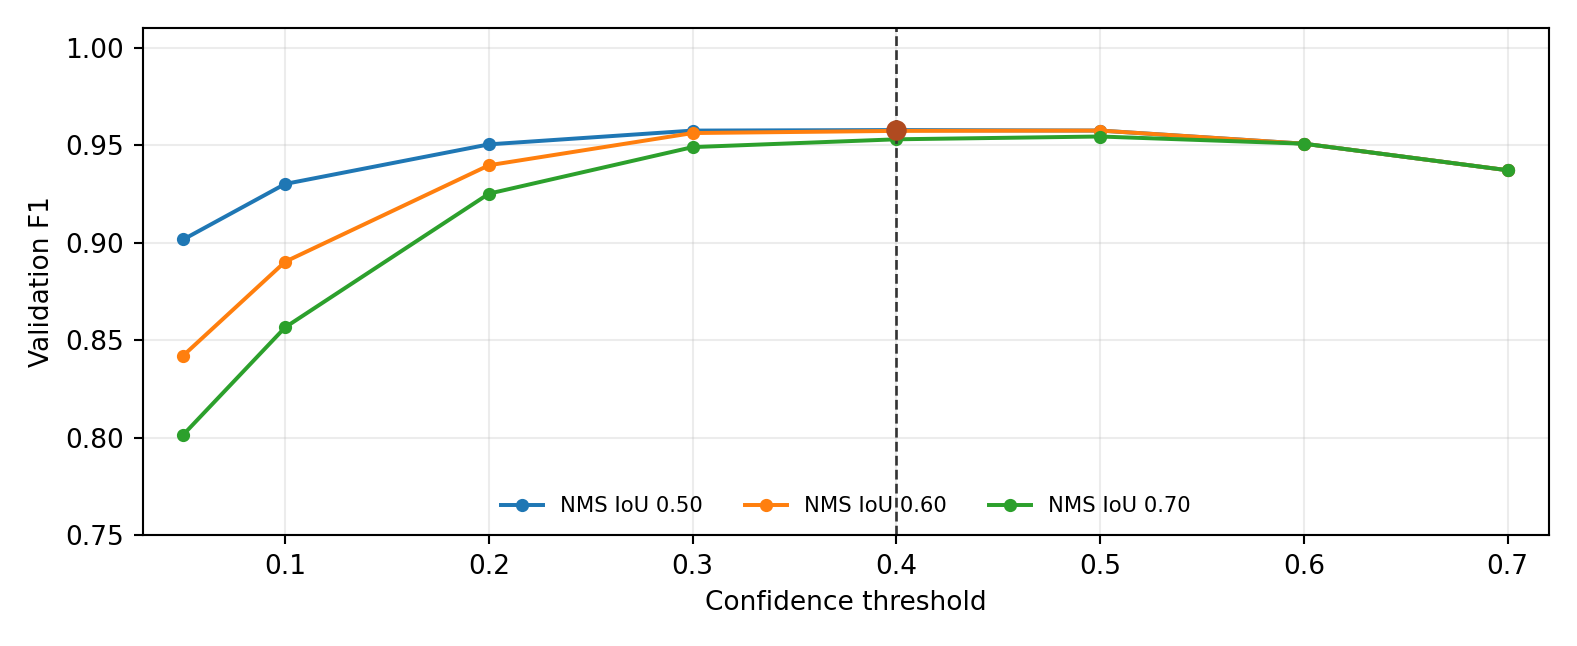
\includegraphics[width=.93\linewidth,height=7cm,keepaspectratio]{figures/M4_threshold_sweep.png}
\caption{Validation threshold sweep reconstructed from the saved threshold-sweep CSV. Split: Oxford validation (1,106 images); detector input: 640 px; confidence 0.05--0.70, NMS IoU 0.50--0.70; selected confidence 0.40 / NMS 0.50.}
\end{figure}
\subsection{Held-out detector results}

{\small\begin{tabularx}{\linewidth}{@{}P{6.9cm} Y@{}}\toprule
Oxford test metric, 1,106 images & Reported value\\\midrule
mAP50 / mAP50--95 & 0.984 / 0.850\\
Cat AP50 / AP50--95 & 0.994 / 0.888\\
Dog AP50 / AP50--95 & 0.973 / 0.812\\
Precision / recall / F1 at conf 0.40, NMS 0.50 & 0.958 / 0.959 / 0.959\\
Matched counts at operating point & TP 1,061; FP 46; FN 45\\
Per-class P/R/F1: cat & 0.980 / 0.983 / 0.982\\
Per-class P/R/F1: dog & 0.948 / 0.948 / 0.948\\
\bottomrule\end{tabularx}}
AP integrates ranked detections across confidence thresholds; the operating-point P/R/F1 above are measured at one chosen threshold and must not be confused with mAP.
\clearpage

\subsection{False positives, false negatives and error analysis}
The archived Oxford test error analysis records 46 false positives and 45 false negatives at 640 px, confidence 0.40, NMS IoU 0.50. Classification and localisation failures can co-occur within an image.

{\small\begin{tabularx}{\linewidth}{@{}Y r Y r@{}}\toprule
FP type & Count & FN type & Count\\\midrule
Localisation (IoU 0.10--0.50) & 34 & Localisation (IoU 0.10--0.50) & 34\\
Species confusion & 10 & Species confusion & 4\\
Localisation and species & 1 & No matching detection & 7\\
Background & 1 & --- & ---\\\bottomrule\end{tabularx}}
Thirty-eight images contain both FP and FN events. A displaced prediction can produce an unmatched predicted box and an unmatched true box under the recorded matching rule. The inspection gallery supports the following plausible, not causally proven, patterns: partial occlusion, clothing, low contrast and loose trimap boundaries.
\begin{figure}[H]\centering
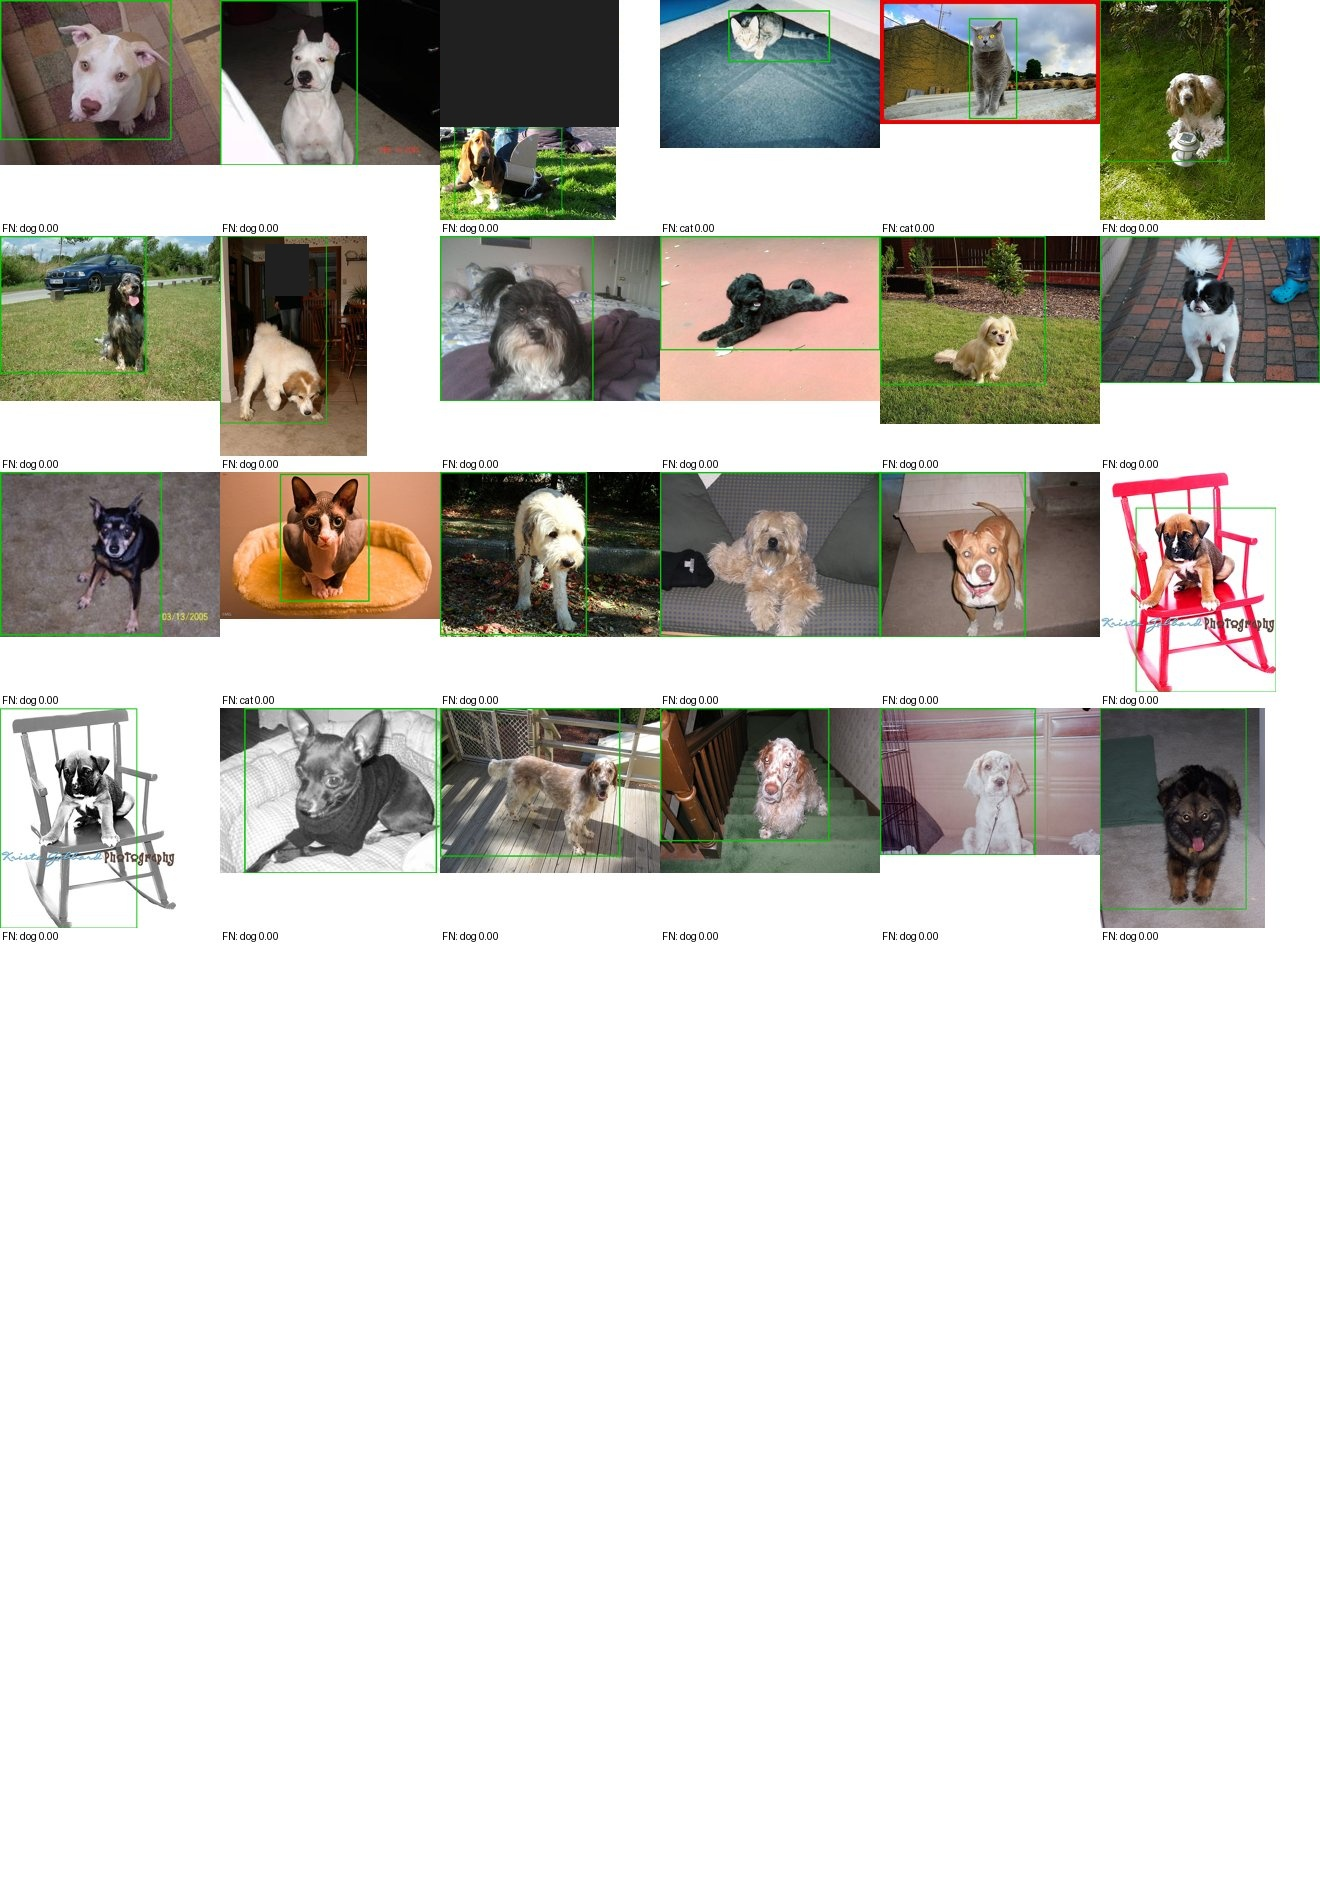
\includegraphics[width=.76\linewidth,height=8.2cm,keepaspectratio]{figures/M4_false_negatives_gallery.jpg}
\caption{Archived false-negative examples. Split: Oxford test; input: 640 px; conf 0.40, NMS IoU 0.50; matching IoU 0.50. Images illustrate difficult localisation, confusion and missed boxes.}
\end{figure}
\begin{figure}[H]\centering
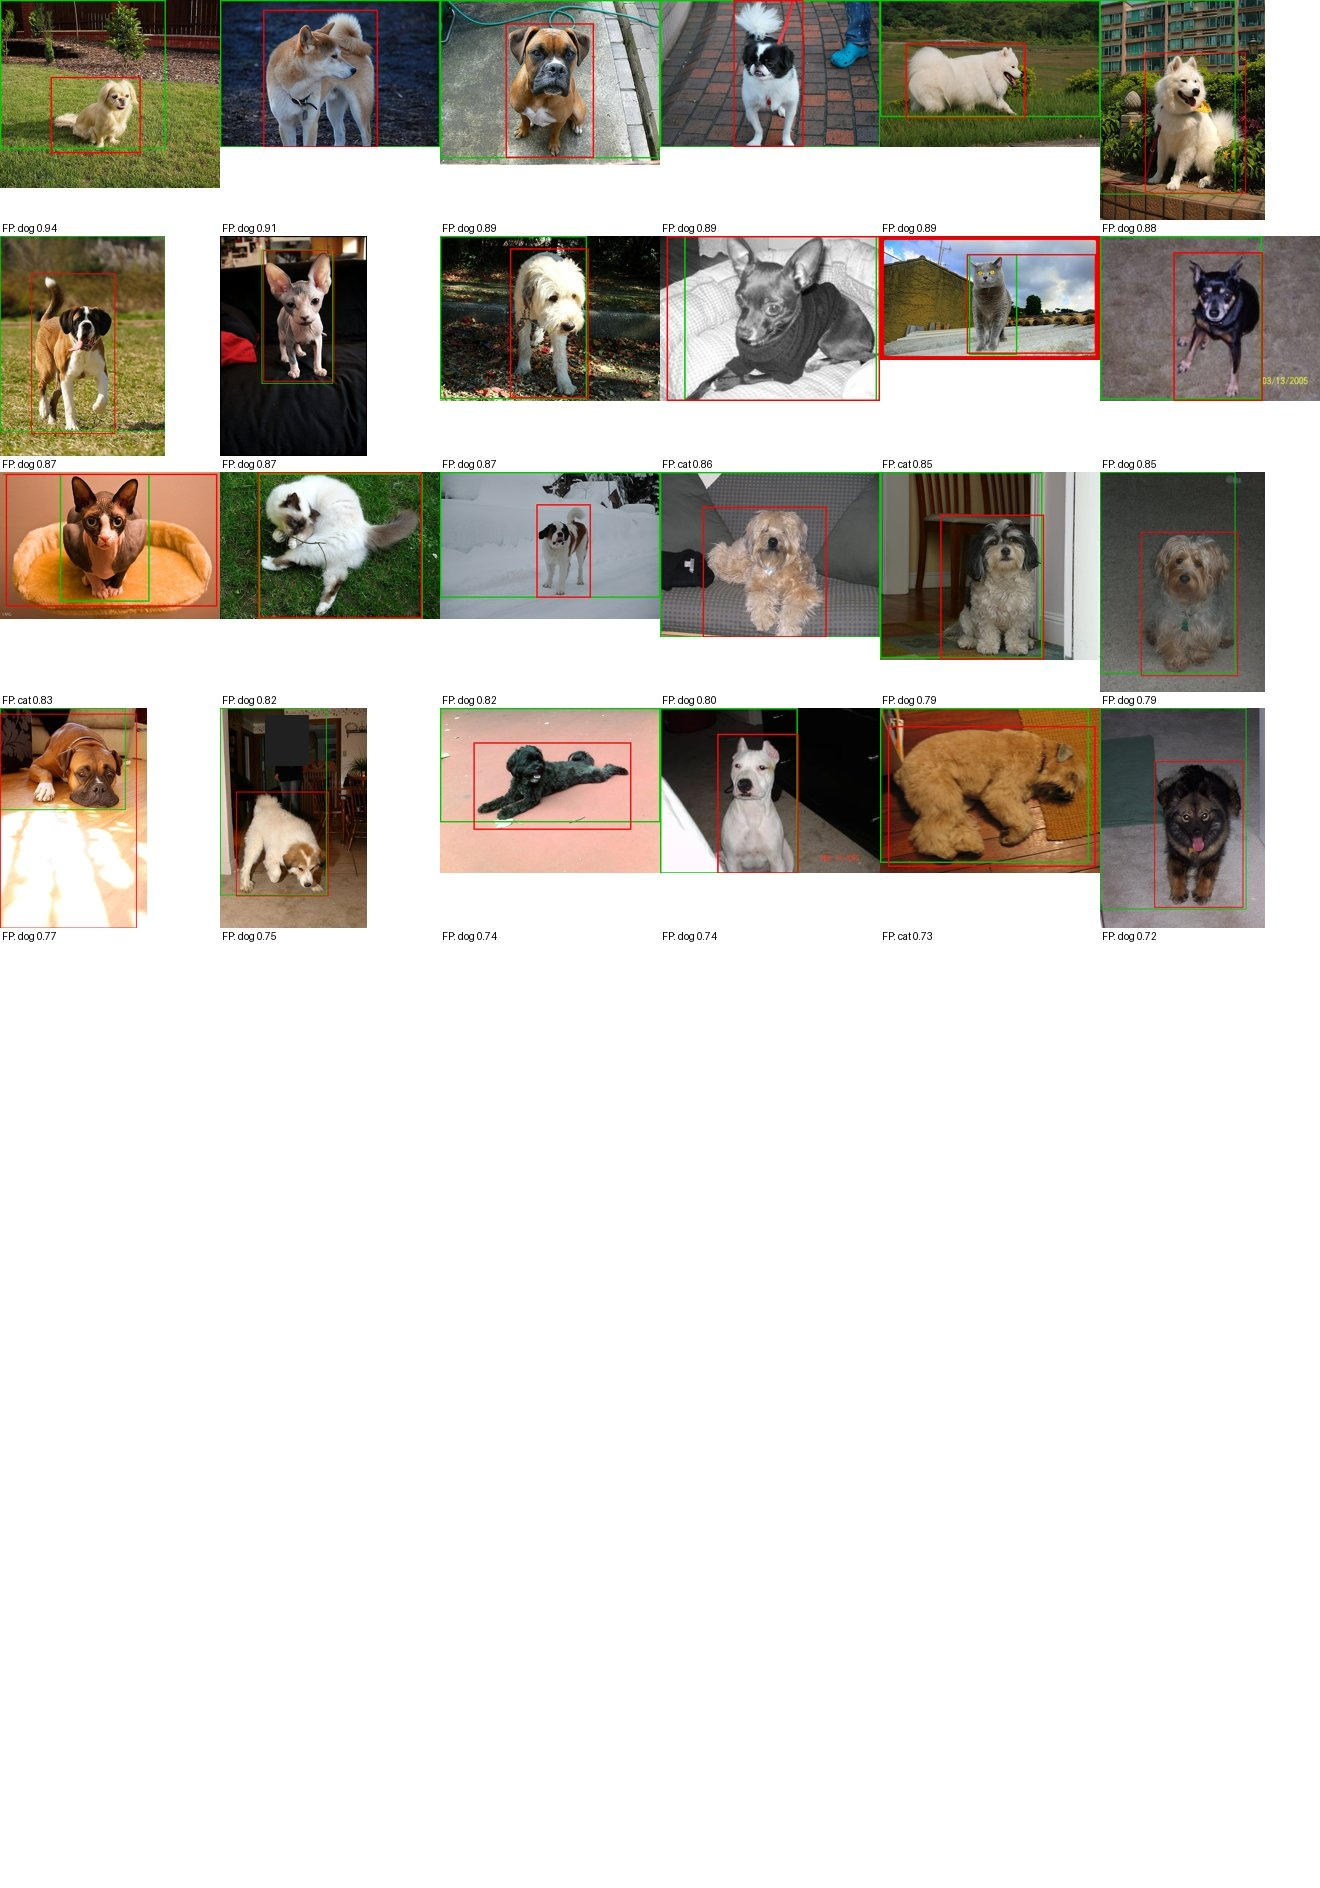
\includegraphics[width=.76\linewidth,height=8.2cm,keepaspectratio]{figures/M4_false_positives_gallery.jpg}
\caption{Archived false-positive examples. Split: Oxford test; input: 640 px; conf 0.40, NMS IoU 0.50; matching IoU 0.50. Most of the 46 false positives are displaced boxes (34) or species confusions (10); one is on background.}
\end{figure}
\textbf{Case study.} A dark Chihuahua wearing clothing (\code{chihuahua_156}) was detected as a cat; the classifier independently returned dog, allowing the integrated rule to refer the photo for disagreement. The clothing explanation is a visual hypothesis. On the Oxford test set seven animal images had no matched detection at all.
\clearpage

\subsection{Previously evaluated team-photo benchmark}
The separate 401-image collection was manually annotated in CVAT, and has \textbf{503 boxes}. It has already been used for supplemental project evaluation; its results are not a new untouched holdout. The recorded detector operating point remained 640 px, confidence 0.40, NMS IoU 0.50.

{\small\begin{tabularx}{\linewidth}{@{}P{7.2cm} Y@{}}\toprule
Team benchmark statistic & Result\\\midrule
mAP50 / mAP50--95 & 0.771 / 0.653\\
Cat AP50 / AP50--95 & 0.840 / 0.703\\
Dog AP50 / AP50--95 & 0.702 / 0.603\\
Precision / recall / F1; 503 annotated animals & 0.885 / 0.732 / 0.801\\
Matches at conf 0.40: TP / FP / FN & 368 / 48 / 135\\
Correct count of animals per photograph & 339 / 401\\
Images with multiple animals, all found & 11 / 52\\
Images with no detection & 13 / 401\\\bottomrule\end{tabularx}}
\begin{figure}[H]\centering
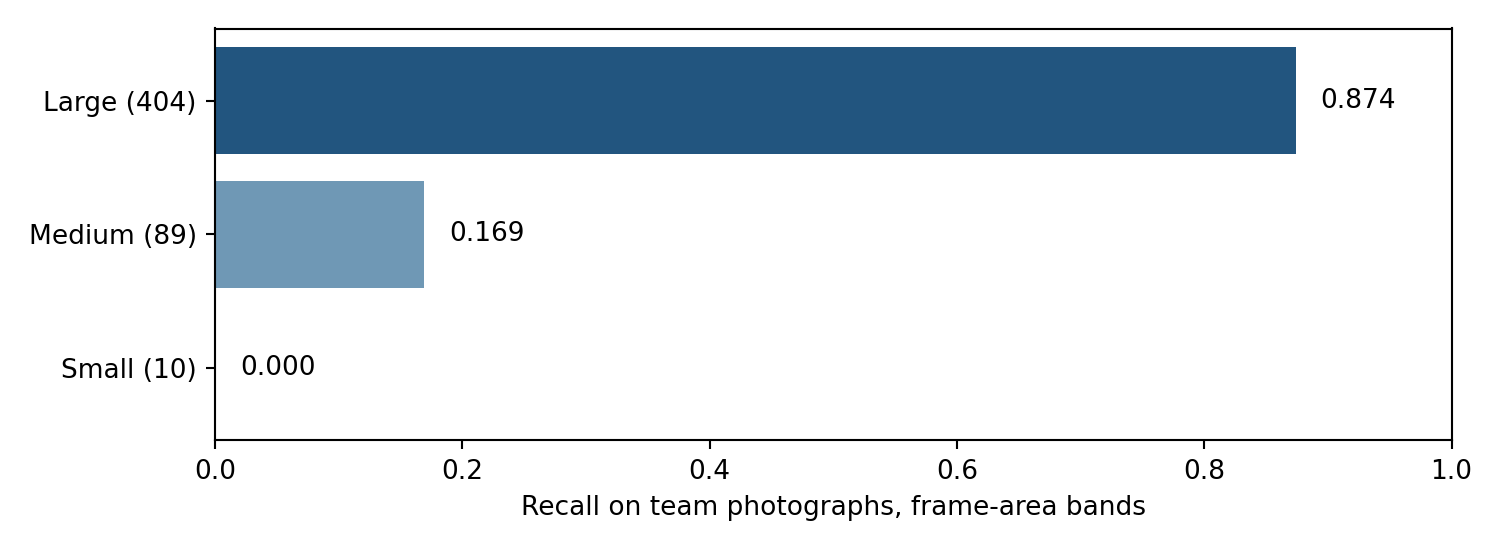
\includegraphics[width=.91\linewidth,height=5cm,keepaspectratio]{figures/M4_size_recall.png}
\caption{Team-set recall by animal box area relative to frame: large $\geq10\%$ ($n=404$), medium 1--10\% ($n=89$), small $<1\%$ ($n=10$). Split: previously evaluated team set; input 640 px; confidence 0.40, NMS 0.50. These are frame-share bands, not COCO pixel-size bands.}
\end{figure}
For comparison, on the Oxford test set 1,105 of the 1,106 boxes fall in the large band (recall 0.959) and only one is medium (detected); Oxford therefore cannot measure small-animal recall, which is why the team-set bands above are the only size evidence. The contrast with Oxford mAP50 (0.984 versus 0.771) is consistent with an application-domain gap, while different populations and annotations also matter. Small or secondary animals are particularly difficult; the ten-image small bin is too limited to estimate universal recall.
\clearpage

\subsection{Video inference demonstration}
The detector was also applied frame by frame to two openly licensed Wikimedia Commons clips; the service itself accepts photographs rather than video.

{\small\begin{tabularx}{\linewidth}{@{}P{4.2cm} r P{2.7cm} Y@{}}\toprule
Video, licence & Frames & Detector mean/p95 & Frames with 0 / 1 / 2+ boxes; labels\\\midrule
Africanis Dogs Resting in Grass (CC0; Umngeni) & 506 & 12.0 / 14.2 ms & 0 / 506 / 0; 506 dog, 0 cat\\
Cat in a Bag (CC BY 2.0; Roger Braunstein) & 510 & 11.3 / 14.6 ms & 222 / 286 / 2; 286 cat, 4 dog\\\bottomrule\end{tabularx}}
\begin{figure}[H]\centering
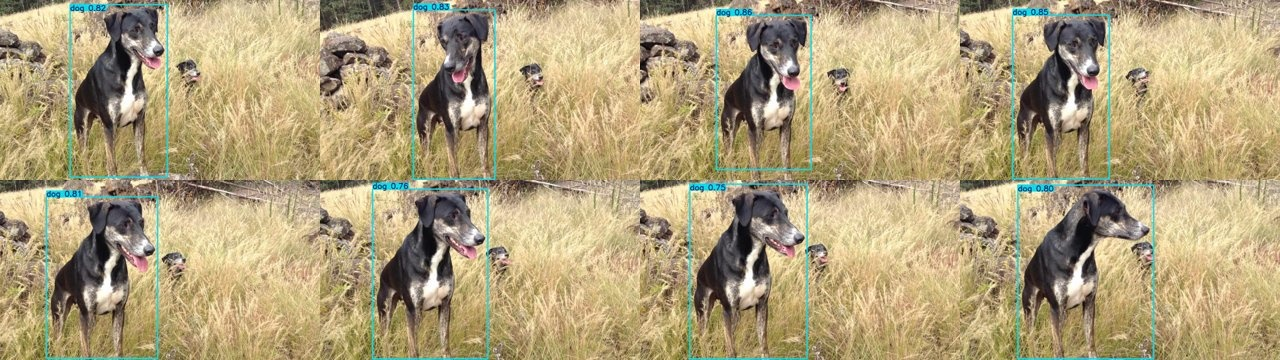
\includegraphics[width=.90\linewidth,height=4.4cm,keepaspectratio]{figures/M4_video_Africanis_Dogs_Resting_In_Grass.jpg}\\[4pt]
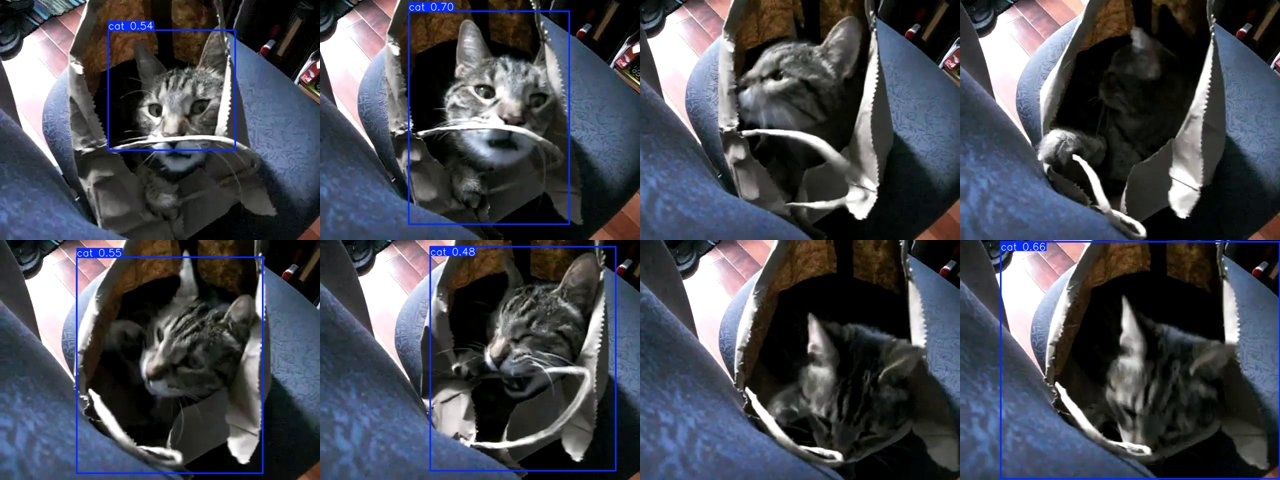
\includegraphics[width=.90\linewidth,height=4.4cm,keepaspectratio]{figures/M4_video_Cat_in_a_Bag.jpg}
\caption{Saved detector video frames; data split: licensed external demo clips; input: 640 px, conf 0.40, NMS IoU 0.50. The partly hidden cat is absent from 222 frames, and 4 detections in this cat-only clip are labelled dog (species errors). The dog clip has no cat labels. Frames are demonstration evidence rather than a new image-level test set.}
\end{figure}
The dog remains visible throughout the first clip. The cat is hidden behind a bag for much of the second, making failure detection a more important observation than aggregate clip accuracy.
\clearpage

\section{Segmentation (M5)\pts{15}}
\subsection{Masks, baseline and model training}
The body-mask target is derived from the Oxford trimap foreground plus ambiguous border. A separate evaluation ignores border pixels, to show sensitivity to the trimap convention. A random subset of 300 Oxford test images was used for the \textbf{SAM 2.1-B} reference, prompted with each image's ground-truth box. This oracle-box input makes SAM a controlled reference, not a direct production alternative. The \textbf{YOLO11s-seg} model was fine-tuned for 40 epochs at 640 px, with confidence 0.25 for the archived mask evaluation.

Training logs: \href{https://wandb.ai/yasser-alhajlah-kaust/smart-pet-vision/runs/3ztpz2tc}{YOLO segmentation 3ztpz2tc}; \href{https://wandb.ai/yasser-alhajlah-kaust/smart-pet-vision/runs/1jb5y453}{SAM reference 1jb5y453}.
\begin{figure}[H]\centering
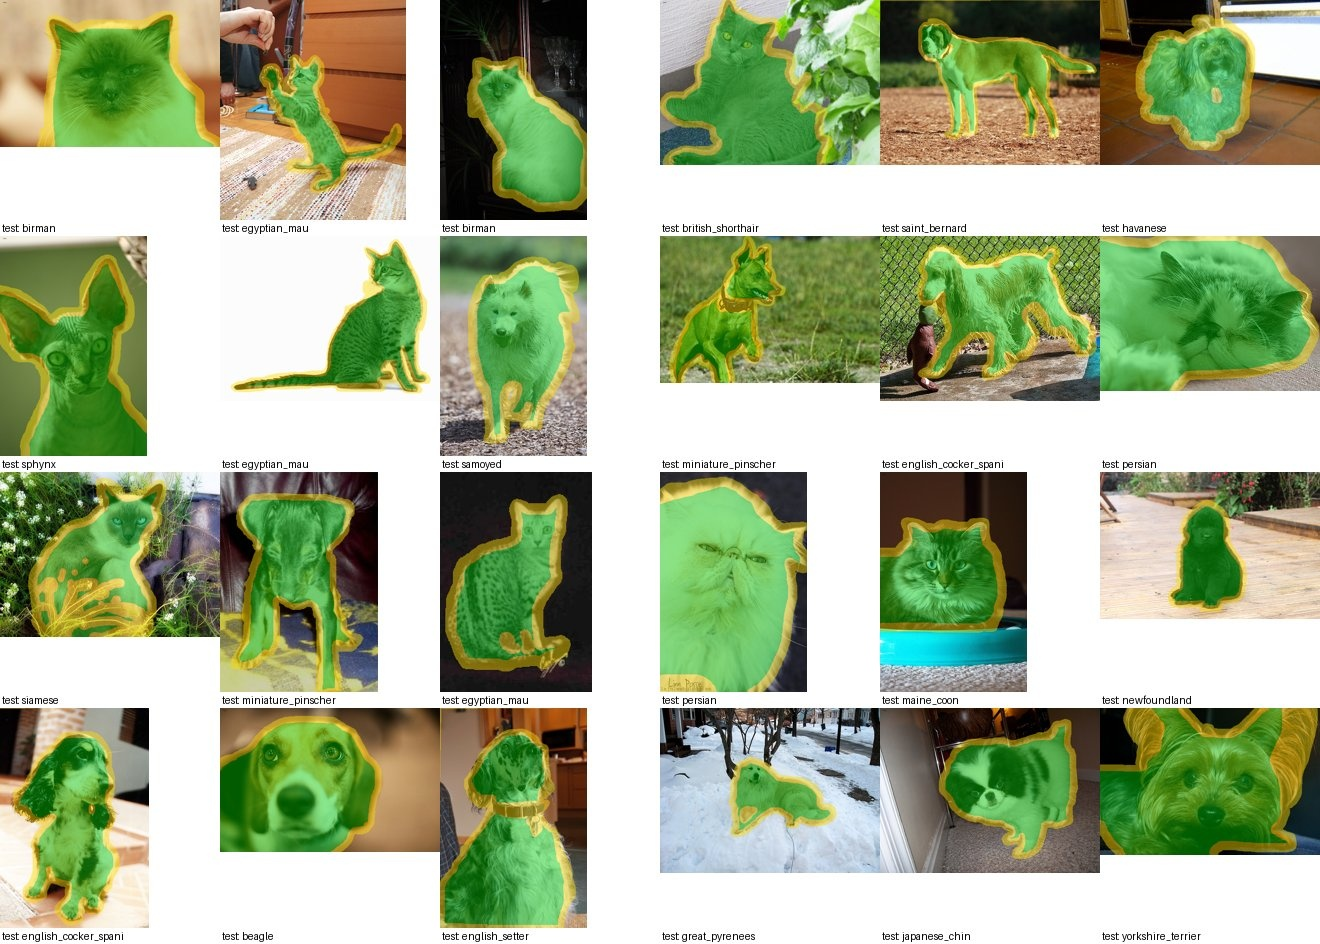
\includegraphics[width=.88\linewidth,height=8.0cm,keepaspectratio]{figures/M5_gt_mask_check.jpg}
\caption{Visual audit of Oxford body-mask targets. Split: Oxford test; resolution: native image / annotation coordinates; threshold: binary trimap foreground plus border. Gallery sampled from saved evidence, not newly annotated.}
\end{figure}
Mask IoU is $|P\cap G|/|P\cup G|$ and Dice is $2|P\cap G|/(|P|+|G|)$ for prediction $P$ and ground truth $G$. The report uses the mean of per-image binary foreground-union scores, while mask mAP is the instance-level class-aware metric.
\clearpage

\subsection{Quantitative evaluation and matched subset}

{\small\begin{tabularx}{\linewidth}{@{}P{5cm} r r Y@{}}\toprule
Model and population & mIoU & Dice & Mask mAP50 / 50--95\\\midrule
SAM 2.1-B, GT-box oracle (test, $n=300$) & 0.812 & 0.883 & Not applicable\\
YOLO11s-seg (test, $n=1,106$) & 0.923 & 0.959 & 0.993 / 0.875\\\bottomrule\end{tabularx}}
For an image-matched comparison, the same 300 test IDs are used for both systems; SAM retains the oracle box while YOLO uses independent model inference:
\begin{figure}[H]\centering
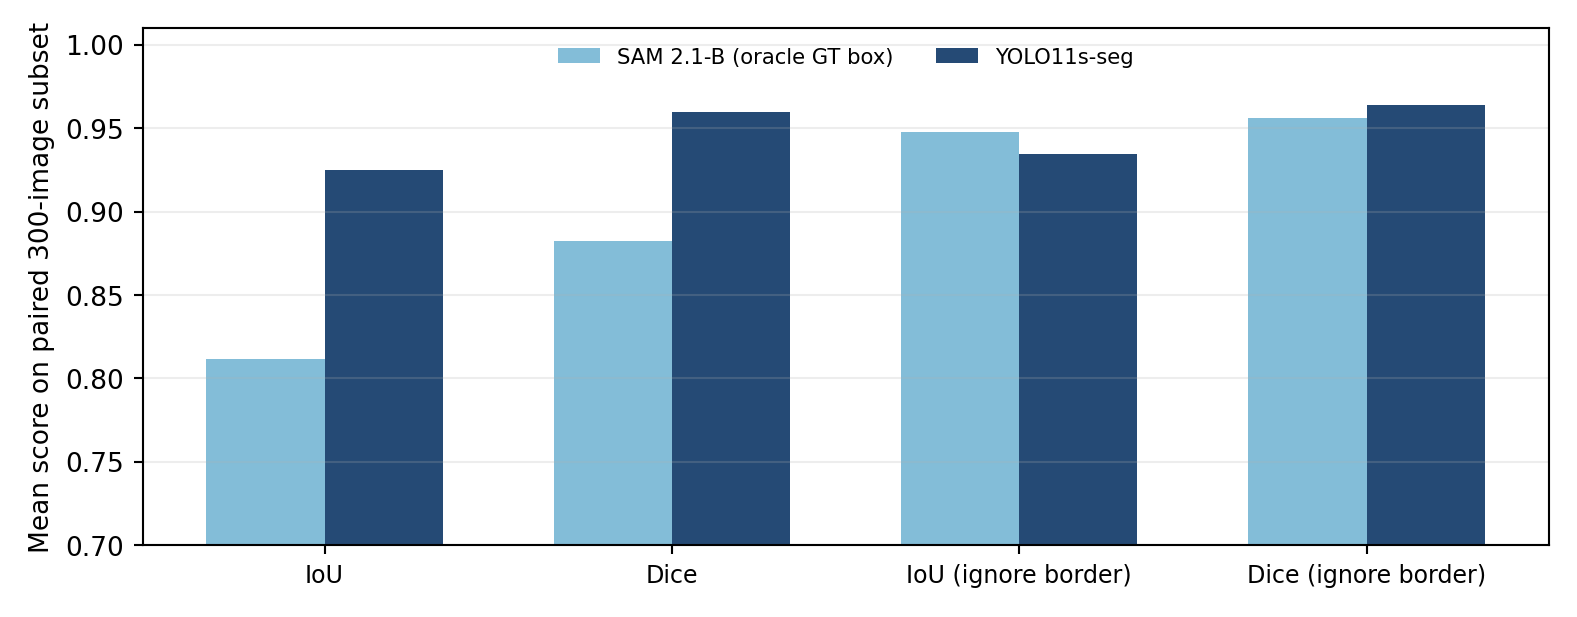
\includegraphics[width=.96\linewidth,height=6.5cm,keepaspectratio]{figures/M5_paired_metrics.png}
\caption{Replot of per-image means from the common 300-image Oxford test subset. YOLO11s-seg input: 640 px, conf 0.25; SAM 2.1-B input: original image, ground-truth box prompt; border-ignored metrics remove ambiguous trimap pixels.}
\end{figure}

{\small\begin{tabularx}{\linewidth}{@{}P{5.0cm} r r r r@{}}\toprule
Matched 300-image protocol & IoU & Dice & IoU, no border & Dice, no border\\\midrule
SAM 2.1-B (oracle box) & 0.8116 & 0.8826 & 0.9476 & 0.9561\\
YOLO11s-seg & 0.9252 & 0.9595 & 0.9342 & 0.9638\\\bottomrule\end{tabularx}}
Differences in box prompts, image scaling and scoring protocol prevent interpreting this as a causal model comparison. The SAM baseline reaches mask IoU $\geq0.8$ on 215/300 primary masks and border-ignored IoU $\geq0.9$ on 278/300 samples. In the YOLO full test set, the lowest reported breed-level mean IoUs include beagle (0.889), miniature pinscher (0.891) and Siamese (0.899).
\clearpage

\subsection{Failure analysis and segmentation limitations}
\begin{figure}[H]\centering
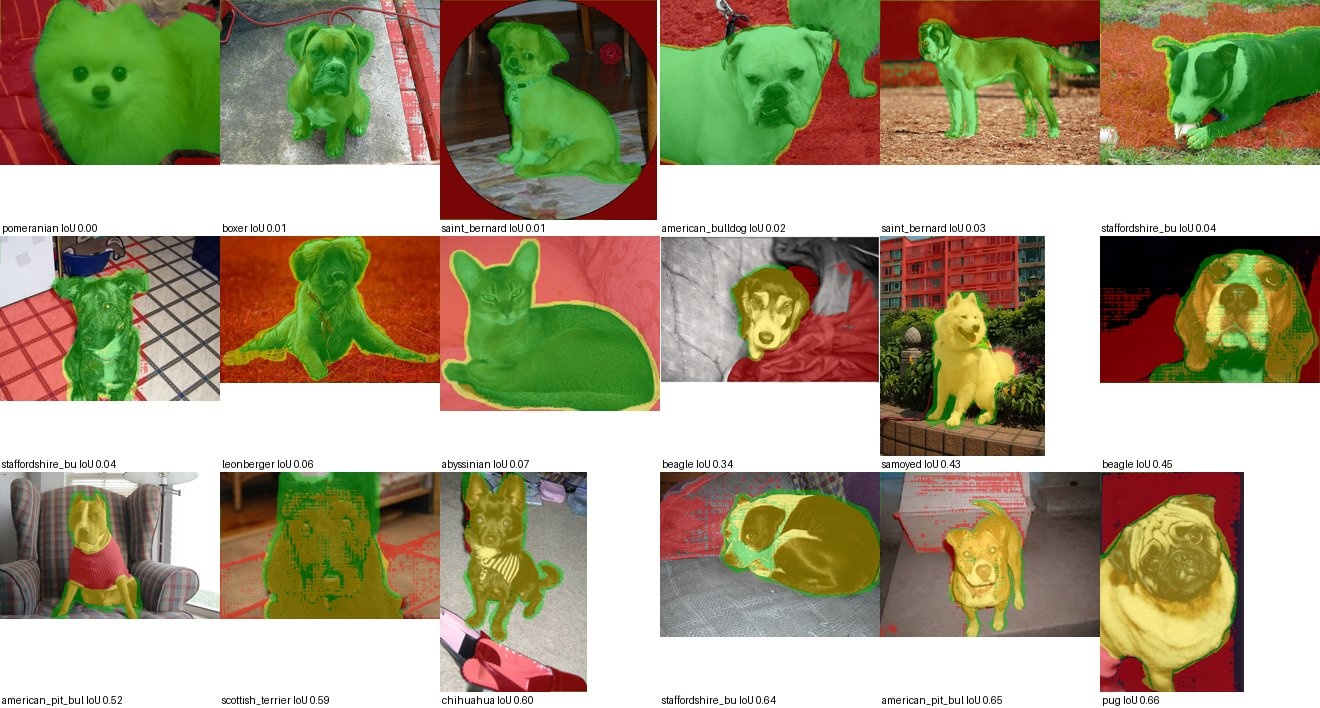
\includegraphics[width=.90\linewidth,height=7cm,keepaspectratio]{figures/M5_sam_baseline_failures.jpg}
\caption{Archived SAM baseline failure examples. Split: Oxford test sampled 300; input: native resolution with ground-truth box prompt; score: binary foreground-union IoU against trimap body masks. Some close-ups lead to background-like masks.}
\end{figure}
\begin{itemize}[leftmargin=1.2em,itemsep=2pt]
\item \textbf{SAM reference failure:} When an oracle box nearly fills the frame, the reference may select background rather than animal. The archive records 12 of 300 primary-mask cases with IoU below 0.5; the very different border-ignored scores show annotation-boundary sensitivity.
\item \textbf{YOLO mask failure:} Similar-colour blankets, clothing and adjacent animals can extend the predicted mask beyond the selected animal, while occlusion can truncate the body. The archived YOLO failure gallery includes scores roughly 0.35--0.67.
\item \textbf{Integration implication:} The mask used for the chosen crop must match \emph{that instance}, not a union of two animals. The current source has explicit instance alignment and dimensionality checks, verified by synthetic regression tests.
\end{itemize}
The private team-photo masks were reviewed in CVAT. Their use in supplemental evaluation does not establish independent real-world performance after later policy changes. Border ambiguity and the absence of verified animal identity remain evaluation limitations.
\clearpage

\section{Integration and deployment (M8)\pts{15}}
\subsection{End-to-end decision workflow}
The application composes the detector, selected animal crop, fine-tuned ResNet-50 species classifier, YOLO body segmenter and referral policy. The selected classifier consumes a 224-pixel crop; detector/segmenter inputs use 640 pixels in the recorded baseline. All weights, thresholds and artifact paths are supplied by \code{runs/manifest.json}.
\begin{figure}[H]\centering
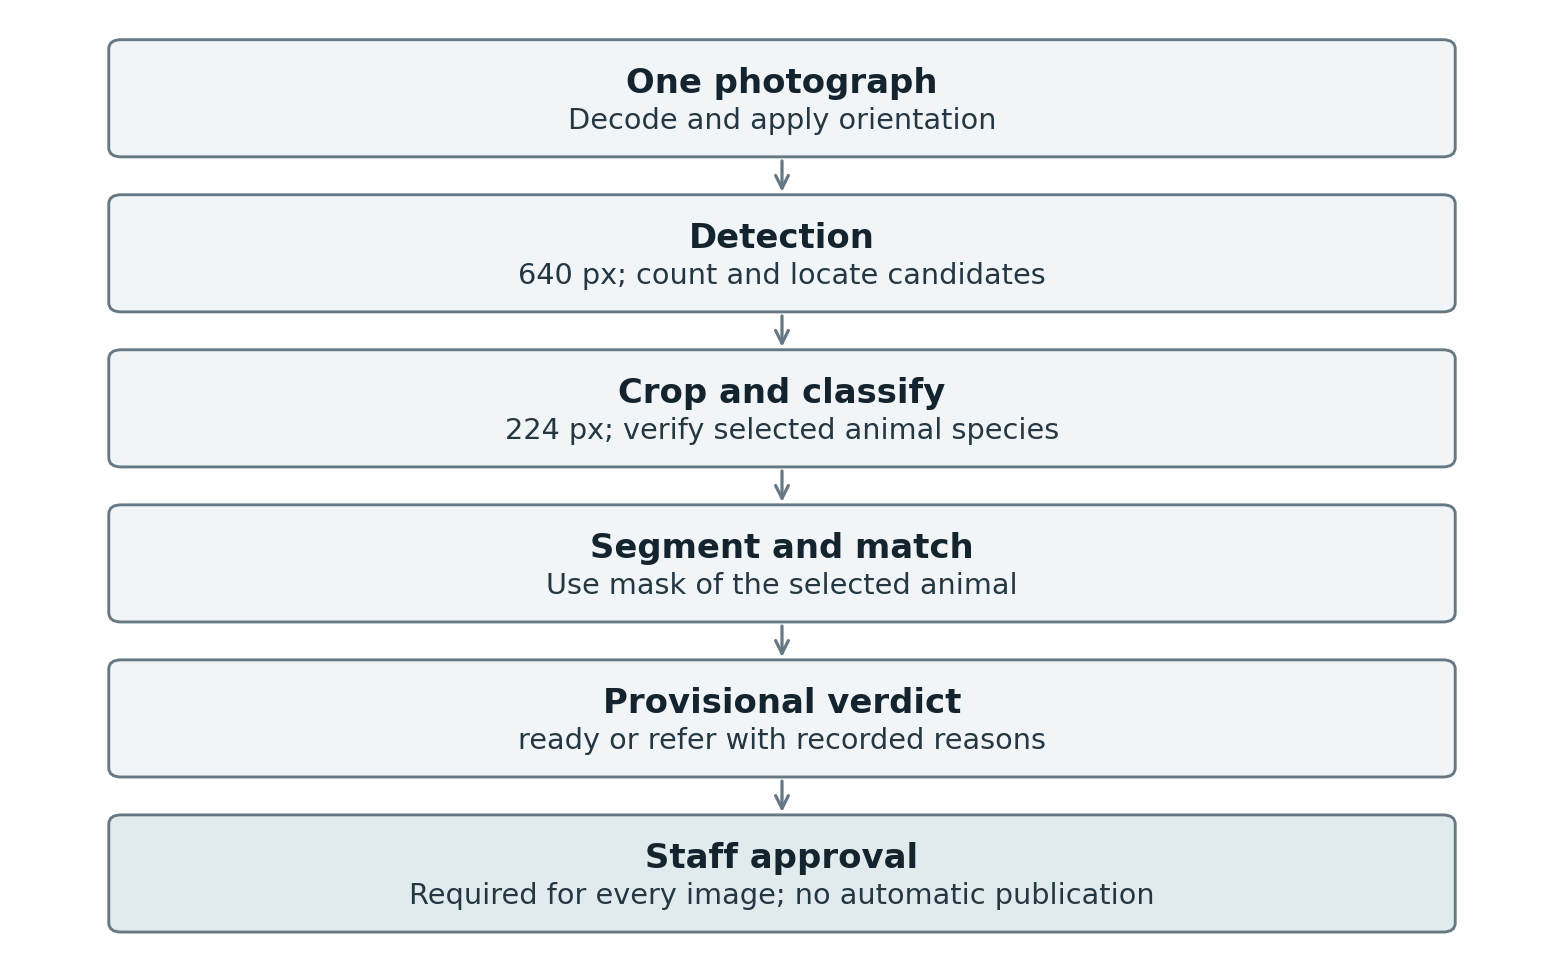
\includegraphics[width=.91\linewidth,height=9cm,keepaspectratio]{figures/pipeline_flow.png}
\caption{Schematic from the reviewed Phase 2 submission package. Source: the integrated pipeline module; detector input 640 px (conf 0.40, NMS 0.50), classifier crop 224 px, temperature 0.05, verification threshold 0.90, minimum matched-mask share 0.05. This is a workflow illustration, not an accuracy result.}
\end{figure}
Referral reasons include no animal, more than one animal, insufficient species confidence, detector/classifier disagreement, an excessively small mask or an unmatched mask. \textbf{Both ready and referred outputs require an explicit staff approval step; automatic publication is disabled.}
\clearpage

\subsection{HTTP service and observed historical benchmarks}
The FastAPI service provides \code{POST /analyze} and \code{GET /health}, with upload and decoded-pixel size limits. Response fields identify the verdict, review reasons, class scores, geometry and per-stage timing. The archived T4 evaluation used 5 warm-up requests and 300 measured requests from a separate HTTP process: 300/300 returned HTTP 200, with p50/p95/p99 \textbf{46/135/178 ms}. Invalid and unreadable file responses were separately exercised.


{\small\begin{tabularx}{\linewidth}{@{}P{4.0cm} P{2.2cm} P{2.2cm} Y@{}}\toprule
Historical backend and platform & p50/p95/p99 & Throughput & Memory\\\midrule
PyTorch models, detector on T4 CUDA & 38 / 61 / 78 ms & 24.1 img/s & 255 MiB PyTorch peak GPU; 1,733 MiB RSS\\
ONNX detector on CPU + other models on T4 & 281 / 364 / 702 ms & 3.3 img/s & 218 MiB PyTorch peak GPU; 1,914 MiB RSS\\\bottomrule\end{tabularx}}
Method: first 50 test images cycled, batch 1, 10 warm-up + 200 timed runs, one process per backend. The two backends do not share the same detector execution device. The selected service implementation uses \textbf{PyTorch}; ONNX is an evaluated diagnostic export, not the deployed detector. Table values come from \code{evidence/M8_benchmark_pytorch.json} and \code{M8_benchmark_onnx_detector.json}. W\&B run fqow5ly7 logged a separate repetition (PyTorch p50/p95/p99 41.9/58.3/92.8 ms, 22.0 img/s; ONNX-detector 286/318/342 ms, 3.4 img/s); both repetitions meet A8 for PyTorch.

\subsection{Export and numerical parity record}
The classifier ONNX numerical check recorded a maximum absolute difference of $2.98\times10^{-7}$, within the 0.001 bound set before the Phase 2 runs (criterion A9a: met). For the detector, the acceptance check recorded a maximum absolute difference of \textbf{0.0018 against the same 0.001 bound applied to the detector (criterion A9b): not met}. A later re-check on four random inputs recorded 0.0020 (also above the bound). On three real letterboxed images the raw-head maximum was 0.0013 and final boxes matched to 0.0001 px, but a wider comparison on 50 real letterboxed test images (CPU for both runtimes, conf 0.40, NMS 0.50) found a raw-head maximum of 0.0027, the same number of detections and the same classes on 98\% of images, and a largest final-box displacement of 28.7 px. The exported detector is therefore not interchangeable with the PyTorch detector at the operating point; the service uses PyTorch.


{\small\begin{tabularx}{\linewidth}{@{}P{5.1cm} P{3cm} Y@{}}\toprule
ONNX verification item & Saved outcome & Evidence scope\\\midrule
Classifier numerical parity & $2.98\times10^{-7}$; pass & Recorded classifier model / CPU\\
Detector numerical parity (A9) & 0.0018 vs. $\le$0.001; \textbf{not met} & \code{M8_onnx_parity.json}, \code{M8_acceptance.csv}\\
Detector raw head, re-check, 4 random inputs & 0.0020; not met & \code{M8_onnx_parity_recheck_4inputs.json}\\
Detector, 3 real images & raw 0.0013; same detections; box shift 0.0001 px & \code{M8_onnx_parity_real_images_3.json}\\
Detector raw head, 50 real images & 0.0027 & \code{M8_onnx_parity_real_images.json}\\
Detector final detections, 50 real images & 98\% same count and classes; max box shift 28.7 px & \code{M8_onnx_parity_real_images.json}\\\bottomrule\end{tabularx}}
The 0.001 bound was set for the classifier before any Phase 2 run (A9) and was extended to the detector (A9b) no later than the first integration run on 17 October; it is not relaxed here. The three-image result is consistent with the 50-image result but too small to show the 2\% of images where the two runtimes disagree. Closing A9 would need an export change (for example FP32 graph without fused post-processing, or comparing at the decoded-box level with a pre-registered tolerance in a new phase) and a re-run.
\clearpage

\subsection{Integrated decisions on the inspected 401-photo collection}
The full team set contains 399 single-species photos (which can contain multiple animals of one species) and two mixed cat/dog images. The most recent archived \emph{real-weight CPU run} recorded the following results, without retraining. This is regression on an already inspected dataset, not a fresh untouched final test.

{\small\begin{tabularx}{\linewidth}{@{}P{7cm} Y@{}}\toprule
Metric / population & Latest recorded CPU value\\\midrule
Single-species correct predictions & 386/399 (96.74\%)\\
Referral decisions, all team photos & 81/401 (20.20\%)\\
Technically ready, all team photos & 320/401\\
Correct species among technically ready & 319/320\\
Multi-animal photos technically ready & 17/52\\
Mixed cat/dog photos technically ready & 0/2\\
Staff approval required; automatic publication & 401/401 required; none permitted\\\bottomrule\end{tabularx}}
\begin{figure}[H]\centering
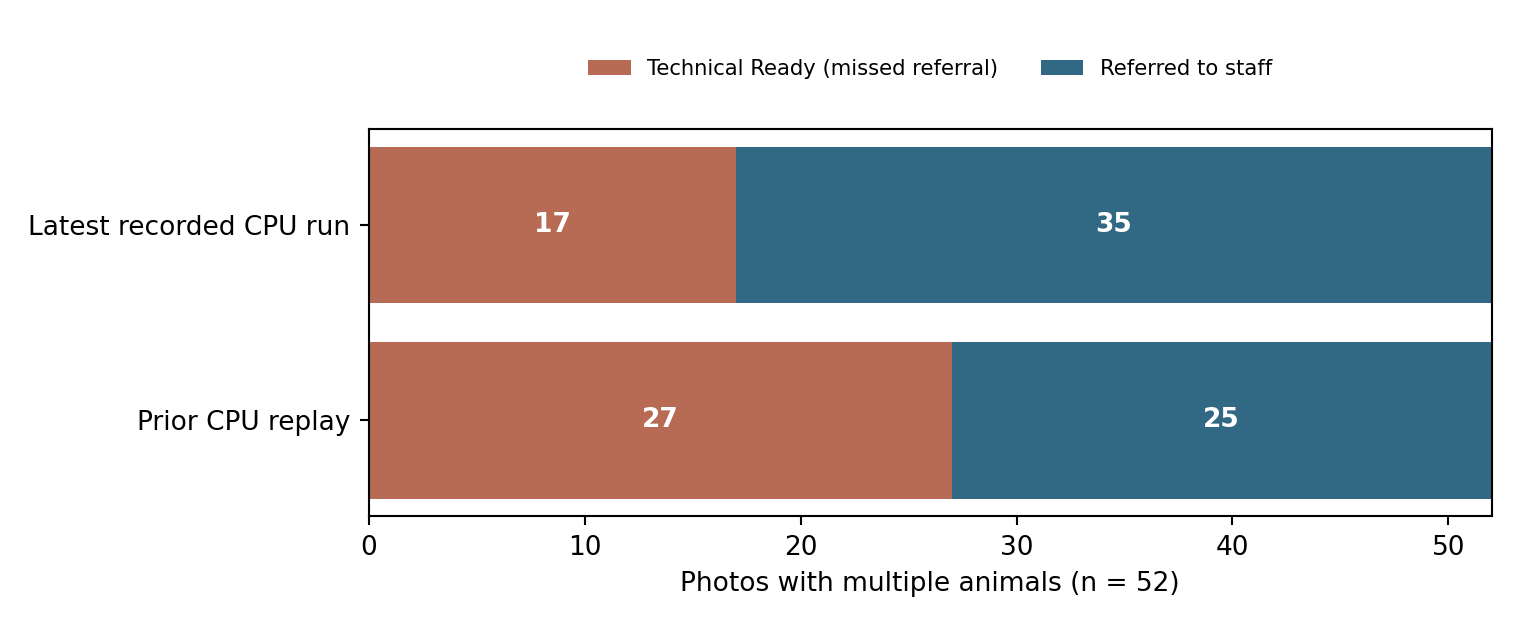
\includegraphics[width=.91\linewidth,height=5.3cm,keepaspectratio]{figures/M8_multi_animal_recorded.png}
\caption{Comparison of two recorded CPU regression snapshots, \emph{not} a controlled one-change experiment: prior replay 27/52 technically ready, latest saved CPU run 17/52. Population: 52 multi-animal photos in the previously evaluated team set; baseline detector 640 px, conf 0.40, NMS 0.50. Different source/runtime snapshots prevent attributing the change to a single patch.}
\end{figure}
Because the referral rule counts \emph{detected} animals, a multi-animal photograph is marked technically ready only when the detector reports a single animal; the 17 such cases are therefore photographs in which secondary animals were missed (consistent with the low medium/small recall above), and staff review must catch them. The CPU run also counts 386/399 correct single-species predictions, one fewer than the 387/399 Phase 1 figure, because it is a later re-run with two changed modules. The CPU results are attributed to their saved runtime configuration, which predates the latest complete source snapshot for two modules. They remain a useful regression record; every technically ready photograph still requires explicit staff approval.
\clearpage

\section{Acceptance criteria and go/no-go decision}
Thresholds A1--A8 and A9a are recorded in the team's integration notebook in the code snapshot of 15 October 2026, before the first Phase 2 training run (W\&B, 17 October); the submitted Phase 1 report states only A1--A2. Row A9b, the same 0.001 bound applied to the detector, was added no later than the first integration run (17 October), and the detector fails it. Values are taken from \code{evidence/M8_acceptance.csv}; splits are the Oxford test split (1,106 images) unless stated.

{\small\begin{tabularx}{\linewidth}{@{}P{0.9cm} Y P{2.0cm} P{1.8cm} P{1.2cm}@{}}\toprule
ID & Criterion (setting) & Value & Target & Met\\\midrule
A1 & Classification accuracy & 0.999 & $\ge$ 0.90 & Yes\\
A2 & Classification macro-F1 & 0.999 & $\ge$ 0.90 & Yes\\
A3 & Detection mAP50 (640 px) & 0.984 & $\ge$ 0.75 & Yes\\
A4 & Detection recall (conf 0.40, NMS 0.50) & 0.959 & $\ge$ 0.80 & Yes\\
A5 & Segmentation mean IoU & 0.923 & $\ge$ 0.75 & Yes\\
A6 & Segmentation mean Dice & 0.959 & $\ge$ 0.85 & Yes\\
A7 & Service success rate (HTTP, PyTorch) & 300/300 & $\ge$ 0.99 & Yes\\
A8 & p95 latency, T4, batch 1, PyTorch & 61.4 ms & $\le$ 2,000 ms & Yes\\
A9a & ONNX max abs diff, classifier & $2.98\times10^{-7}$ & $\le$ 0.001 & Yes\\
A9b & ONNX max abs diff, detector & 0.0018 & $\le$ 0.001 & \textbf{No}\\\bottomrule\end{tabularx}}

\textbf{Decision.} \emph{Go} for a staff-supervised demonstration with the PyTorch backend: A1--A8 and A9a are met. \emph{No-go} for serving the ONNX detector: A9b is not met and final boxes moved by up to 28.7 px on real images. On the team photographs, which are not the acceptance population, detector recall is 0.732 and dog recall 0.651 (both below the 0.80 recall target if it were applied there); this limits use to supervised review, where every photograph is approved by staff.

\section{Reproducibility and evidence tracking}\label{sec:repro}

{\small\begin{tabularx}{\linewidth}{@{}P{4.0cm} Y@{}}\toprule
Record & How to reproduce or verify\\\midrule
Dataset and partitions & Oxford-IIIT Pet; 7,335 retained; seed 42; group-aware 5,123/1,106/1,106; private photos stay outside public archives\\
Model configuration & \code{configs/config.yaml}, \code{runs/manifest.json}, pinned requirements and saved checkpoint paths\\
Detection artifacts & W\&B \href{https://wandb.ai/yasser-alhajlah-kaust/smart-pet-vision/runs/2seovilv}{2seovilv}; \code{M4_operating_point.json}, sweep CSV, test and team metrics\\
Segmentation artifacts & W\&B \href{https://wandb.ai/yasser-alhajlah-kaust/smart-pet-vision/runs/3ztpz2tc}{3ztpz2tc}; SAM \href{https://wandb.ai/yasser-alhajlah-kaust/smart-pet-vision/runs/1jb5y453}{1jb5y453}; paired 300 image scores\\
Runtime artifacts & W\&B \href{https://wandb.ai/yasser-alhajlah-kaust/smart-pet-vision/runs/fqow5ly7}{fqow5ly7} (HTTP check, 300/300; a separate benchmark repetition); benchmark table values from \code{evidence/M8_benchmark_*.json}; pipeline manifest\\
Current source provenance & 30 of 30 archived source files matched the saved SHA256 manifest\\
Real-weight model versions & Detector \code{best.pt}, segmenter \code{best.pt}, classifier \code{finetune.pt}; model fingerprints recorded with the evaluation archive\\
Reproduction workflow & \code{notebooks/03_detection.ipynb}, \code{04_segmentation.ipynb} and \code{05_integration.ipynb} in \code{smart-pet-vision/phase2/} of the GitHub repository; all 30 snapshot files were committed unchanged (SHA-256 match); the current version differs in two of them: \code{src/spv/pipeline.py} (opt-in v0.4 multi-animal review, off by default) and \code{notebooks/01_data_preparation.ipynb} (one wording change in a markdown cell) and the unit tests pass (49; 83 with the opt-in v0.4 multi-animal review)\\\bottomrule\end{tabularx}}
\subsection*{What can and cannot be reproduced from this ZIP}
The accompanying Overleaf ZIP is \emph{report source and selected, privacy-reviewed illustrations}, in the same style as the submitted Phase 1 ZIP. It also includes bounded CSV/JSON evidence and manifests. It does \textbf{not} redistribute Oxford image archives, private team photographs, 100+ MB weight files or full training outputs. The separate repository and private Drive evidence are needed to rerun inference.

Saved-metric verification is distinct from model retraining. Source checks, trained-weight CPU observations and historical T4 logs provide complementary reproducibility evidence. The previously inspected team photos are treated as a supplementary regression dataset, separate from the held-out Oxford test split.
\clearpage

\section{Submission checklist}
The requirements below follow the October 2026 \emph{Capstone Project Guidelines UPDATED}, Table 5 (p.~6) and Table 6 (p.~7). These checks concern evidence presence and truthful interpretation, not instructor-awarded credit.
\begin{itemize}[leftmargin=1.45em,itemsep=6pt]
\item[$\checkmark$] M4: body boxes converted and sample reviewed; held-out mAP50/mAP50--95 and per-class AP recorded.
\item[$\checkmark$] M4: validation conf/NMS sweep with specified selection rule; per-class P/R/F1, FP/FN breakdown and case study.
\item[$\checkmark$] M4: image and licensed-video demonstrations, with sources, input sizes and thresholds in captions.
\item[$\checkmark$] M5: ground-truth trimaps reviewed; SAM oracle-box baseline and fine-tuned YOLO masks compared.
\item[$\checkmark$] M5: full-test mask IoU/Dice and mask mAP, plus paired 300-image protocol and failure cases.
\item[$\checkmark$] M8: manifested end-to-end workflow; FastAPI endpoints; historical warm-up/timed latency, throughput and memory.
\item[$\circ$] M8: ONNX export and numerical check recorded; classifier within 0.001; \textbf{detector A9 not met (0.0018--0.0020)}, reported as a no-go for the ONNX detector.
\item[$\checkmark$] M8: acceptance table against criteria set before the Phase 2 runs, and an explicit go/no-go decision.
\item[$\checkmark$] M8: adoption-photo referral policy documented; all photos require human approval, regardless of verdict.
\item[$\checkmark$] Data privacy: private team originals excluded from this Overleaf source ZIP; illustrated galleries from saved reference assets.
\item[$\checkmark$] Evidence origin is traceable: experimental metrics, supplementary regression and execution-environment measurements are identified separately.
\item[$\checkmark$] Deliverable scope is explicit: the Phase 2 report presents evaluated models and the staff-supervised PyTorch workflow; the group demonstration is a separate course component.
\end{itemize}
\subsection*{Provenance note}
For this report, the benchmark figures are generated from \emph{existing saved CSV/JSON values}; qualitative galleries are taken from archived figure assets. Figure captions state data population, resolution and applicable thresholds. The submitted Phase 1 results are not altered or reclassified as Phase 2 model performance.
\clearpage

\section{Self-assessment}
This table is a \emph{team preparation checklist}, not a claim of an instructor's grade. Phase 2 is 45 points, divided into M4, M5 and M8 at 15 points each. The later presentation is a separate 15 points.

{\small\begin{tabularx}{\linewidth}{@{}P{3.1cm} P{1.0cm} Y P{3.5cm}@{}}\toprule
Criterion & Points & Strongest supporting evidence & Scope of assessment\\\midrule
M4 Detection & 15 & Label verification, YOLO11s training, conf/NMS sweep, Oxford mAP, FP/FN and video cases & Held-out Oxford and supplementary team benchmark\\
M5 Segmentation & 15 & SAM 300-image reference, YOLO segmentation, IoU/Dice/mask mAP and matched subset & Oracle-box SAM and independent YOLO comparison clearly distinguished\\
M8 Integration & 15 & End-to-end PyTorch workflow, recorded HTTP checks, T4 timings, acceptance table and human-review policy; ONNX detector parity (A9b) not met & Staff-supervised inference and numerical export evaluation\\
\midrule
Phase 2 total & 45 & Module evidence assembled for instructor assessment & Grades are awarded by the instructor\\
Final presentation & 15 & Pipeline demonstration material and experiment records & A separate presentation deliverable\\\bottomrule\end{tabularx}}
\subsection*{Application and demonstration scope}
The integrated \textbf{PyTorch staff-review application} combines established detection and segmentation performance with documented HTTP response and T4 inference measurements. The detector and segmenter meet the team's recorded Oxford accuracy targets. The application produces traceable review recommendations; publication authority remains with shelter staff for every photograph.
\clearpage

\section{Obstacles, next actions and conclusion}

{\small\begin{tabularx}{\linewidth}{@{}P{3.3cm} P{1.2cm} Y P{2.3cm}@{}}\toprule
Engineering consideration & Module & Implemented response & Evidence\\\midrule
Full-body versus head boxes & M4 & Derive body boxes from trimaps; inspect labels and coordinate round trips & Annotation review record\\
Variable scale and occlusion & M4/M8 & Evaluate recall by frame-area band and apply staff-review decisions & Detection benchmark and decision outputs\\
Mask boundary conventions & M5 & Report standard and border-ignored scores; associate masks by instance & Paired 300-image evaluation\\
Multiple-animal decisions & M8 & Trigger referral for multiple detected/segmented instances; staff approval remains mandatory & Integrated workflow and tests\\
ONNX export verification & M8 & Detector failed A9 (0.0018 $>$ 0.001); keep PyTorch in service, no-go for ONNX detector & \code{M8_acceptance.csv}\\
Data provenance and privacy & M1/M8 & Keep private images out of the public report package; identify the supplementary set & Audited data and metadata\\\bottomrule\end{tabularx}}

\subsection*{Conclusion}
The historical YOLO11s detector achieves \textbf{0.984 mAP50} (0.850 mAP50--95) on Oxford, while the YOLO11s-seg model reaches \textbf{0.923 mean mask IoU}, \textbf{0.959 Dice} and \textbf{0.875 mask mAP50--95}. Together with the previously selected fine-tuned classifier, they form a functional staff-review pipeline whose observed T4 and HTTP benchmarks support academic demonstration.

The supplementary 401-image benchmark provides additional insight into referral behaviour under varied pet-photograph conditions. The integrated workflow uses agreement, confidence, animal count and segmentation evidence to support staff review, while retaining mandatory human approval of every listing. Future evaluation can extend the evidence to new shelter photographs without changing the reported Phase 2 measurements.

\textbf{Final scope:} This is an academically evaluated image review assistant, not an autonomous publishing agent, a veterinary diagnostic tool or an individual-animal identification system.
\clearpage

\appendix
\section{Dataset and operational model card summary}

{\small\begin{tabularx}{\linewidth}{@{}P{4.1cm} Y@{}}\toprule
Field & Record\\\midrule
Public source & Oxford-IIIT Pet (Parkhi et al., 2012), recorded licence CC BY-SA 4.0; 7,349 received; 14 excluded; 7,335 retained\\
Train / validation / test & 5,123 / 1,106 / 1,106; breed-stratified near-duplicate groups; seed 42\\
Detector and segmenter labels & Whole-body boxes and foreground-plus-border masks derived from trimaps\\
Private supplementary set & 401 images: 178 cat, 221 dog and 2 mixed; 503 annotated animals; 52 multi-animal photographs\\
Data governance & Original Oxford and private images are not redistributed in the public report source; group/MD5 leakage prevented for observed duplicate relation\\
Intended users & Adoption and shelter staff reviewing candidate listing photographs\\
Outputs & Detected box and class, selected species/classifier confidence, matched mask, review reasons, timings\\
Prohibited deployment & Automatic publication, human or animal tracking/identity, medical use, other species, unsupervised public decisions\\
Key cautions & Small animals, occlusion, close animals, domain shift, overconfident individual errors, possible identity leakage\\\bottomrule\end{tabularx}}
The reported team-collected images have documented team consent/provenance and metadata handling but no independent certification. The 401-image collection was inspected during development and therefore cannot be used as a fresh untouched test for later modifications.
\section{Evidence index and references}

{\small\begin{tabularx}{\linewidth}{@{}P{3.4cm} Y@{}}\toprule
Reference & Exact origin or location\\\midrule
Official assessment & \emph{Capstone Project Guidelines UPDATED} (October 2026), Tables 2, 5, 6, pp.~3, 6, 7\\
Acceptance criteria origin & Team code snapshot \code{smart-pet-vision.zip} (Drive, uploaded 15 October 2026), \code{notebooks/05_integration.ipynb}, table A1--A9; first Phase 2 W\&B runs created 17 October 2026\\
Submitted Phase 1 source & \code{SmartPetVision_Phase1_Overleaf_Source(2).zip}, \code{main.tex}; submitted 16-page PDF\\
Phase 2 archive & \code{SmartPetVision_Phase2_Complete_Reviewed_30Oct2026.zip}; preserved \code{evidence/M4_*}, \code{M5_*}, \code{M8_*}\\
Later real-weight CPU record & \code{Model_Repair_Verification_30Oct2026/summary.json}; source hash differences explicitly noted\\
Recorded integration evidence & \code{evidence/M8_*}; HTTP, latency, model manifest and export comparisons\\
Oxford dataset & \url{https://www.robots.ox.ac.uk/~vgg/data/pets/}\\
Ultralytics metrics & \url{https://docs.ultralytics.com/guides/yolo-performance-metrics/}\\
ONNX Runtime & \url{https://onnxruntime.ai/docs/performance/model-optimizations/graph-optimizations.html}\\\bottomrule\end{tabularx}}
\subsection*{Research references}
\begin{enumerate}[leftmargin=1.45em,itemsep=2pt]
\item Parkhi, O. M., Vedaldi, A., Zisserman, A. and Jawahar, C. V. (2012). \emph{Cats and Dogs}. CVPR. Oxford-IIIT Pet dataset.
\item Kirillov, A. et al. (2023). \emph{Segment Anything}. ICCV. The archived project reference uses SAM 2.1-B.
\item Guo, C., Pleiss, G., Sun, Y. and Weinberger, K. Q. (2017). \emph{On Calibration of Modern Neural Networks}. ICML.
\end{enumerate}
\end{document}
